%%%%%%%%%%%%%%%%%%%%%%%%%%%%%%%%%%%%%%%%%%%%%%%%%%%%%%%
% A template for Wiley article submissions.
% Developed by Overleaf. 
%
% Please note that whilst this template provides a 
% preview of the typeset manuscript for submission, it 
% will not necessarily be the final publication layout.
%
% Usage notes:
% The "blind" option will make anonymous all author, affiliation, correspondence and funding information.


\documentclass[alpha-refs]{wiley-article}


% Add additional packages here if required
\usepackage{siunitx}

\usepackage{amsmath}
\usepackage{amssymb}
\newcommand{\rr}{ {\cal R}_0 }						% dispersion parameter

% Update article type if known
\papertype{Original Article}
% Include section in journal if known, otherwise delete
\paperfield{Journal Section}

\title{On the prior modelling for the basic reproductive ratio}

% List abbreviations here, if any. Please note that it is preferred that abbreviations be defined at the first instance they appear in the text, rather than creating an abbreviations list.
\abbrevs{ABC, a black cat; DEF, doesn't ever fret; GHI, goes home immediately.}

% Include full author names and degrees, when required by the journal.
% Use the \authfn to add symbols for additional footnotes and present addresses, if any. Usually start with 1 for notes about author contributions; then continuing with 2 etc if any author has a different present address.
\author[1,3\authfn{1}]{Luiz Max Carvalho}
\author[2\authfn{1}]{Marcio Marciel Bastos}
\author[3]{Daniel A. Villela}
\author[3]{Leonardo S. Bastos}
\author[2]{Fl\'avio Code\c{c}o Coelho}

\contrib[\authfn{1}]{Equally contributing authors.}

% Include full affiliation details for all authors
% \affil[1]{Department of Statistics, Federal University of Minas Gerais, Belo Horizonte, Brazil.}
\affil[1]{School of Biological Sciences, University of Edinburgh, Edinburgh, UK.}
\affil[2]{School of Applied Mathematics, Get\`ulio Vargas Foundation, Rio de Janeiro, Brazil.}
\affil[3]{Scientific Computing Programme (PROCC), Oswaldo Cruz Foundation, Rio de Janeiro, Brazil.}

\corraddress{Luiz Max Carvalho, Scientific Computing Programme (PROCC), Oswaldo Cruz Foundation, Rio de Janeiro, Brazil.}
\corremail{lmax.procc@gmail.com}


\fundinginfo{Funder One, Funder One Department, Grant/Award Number: 123456, 123457 and 123458; Funder Two, Funder Two Department, Grant/Award Number: 123459}

% Include the name of the author that should appear in the running header
\runningauthor{Carvalho et al.}

\begin{document}

\maketitle

\begin{abstract}

The basic reproductive number, $\rr$, is a central quantity in theoretical epidemiology, defining the threshold between disease-free equilibria and epidemics.
$\rr$ can usually be written as a ratio between the rate of creation of infected individuals and the rate of removal of infected individuals.
Bayesian inference for epidemic models usually proceeds by assigning Gamma or log-normal priors to these rates, obtaining posterior distributions and often computing their ratio to recover a posterior distribution for $\rr$.
In this paper we show that these modelling choices lead to induced distributions on the quantity of interest ($\rr$) that have poor statistical properties.
We propose new classes of priors and also extend the usual approach by correcting the distribution of $\rr$ to explicitly consider the population size $N$.
Our findings show that care is needed when constructing priors for inference of epidemic models to ensure valid conclusions about the quantities of interest. 
% Please include a maximum of seven keywords
\keywords{Epidemic models, basic reproductive number, prior modelling, Bayesian inference.}
\end{abstract}

\begin{itemize}
 \item Collect the models that give the gamma ratio for the $\rr$ ;
 \item select studies and data sets to evaluate;
 \item study moment-matching priors with better tail properties
 \item Question: does restricting the support of $f_{\rr}(r)$ to $[0, N]$ lead to improved inference?
 \item Derive $E[\rr]$, $\text{Var}(\rr)$, etc, with the support correction.
\end{itemize}

\section{Epidemic models}

What are epidemic models?

Why they are useful?

$\rr$ is represents the threshold between epidemic and disease-free equilibria.
Useful summary; often reported

\paragraph{SIR model}

\begin{eqnarray*}
\frac{dS}{dt}&=& - \beta SI\\
\frac{dI}{dt}&=&  \beta SI - \gamma I\\
\frac{dR}{dt}&=& \gamma I 
\end{eqnarray*} 
where  $S(t) + I(t) + R(t) = N \: \forall t$, $\beta$ is the transmission (infection) rate and $\gamma$ is the recovery rate.
The basic reproductive number is 

\begin{equation}
\label{eq:r0def}
\rr = \frac{\beta N}{\gamma}. 
\end{equation}

\section{Bayesian estimation of transmission and recovery rates}

~\citep{Coelho2011}



LITERATURE REVIEW

\begin{equation}
 \label{eq:posterior}
 p(\boldsymbol\theta | \boldsymbol Y) \propto \mathcal{L}(\boldsymbol Y | \boldsymbol \theta)\pi(\boldsymbol\theta)
\end{equation}


\subsection{The induced prior on $\rr$}

When constructing prior distributions it is important to consider the effects of these prior distributions on quantities of interest (q.o.i.) in the model, particularly when these are non-linear transforms of the parameters~\citep{Seaman2012}.
Even if a prior distribution seems uninformative on the scale of the parameter it was designed to model, the~\textbf{induced} distribution on the q.o.i. might be informative.

In this section we expand the discussion in Section 2.4 of~\cite{Clancy2008} about the induced distribution on $\rr$ when using Gamma priors on $(\gamma, \beta)$ and also consider the case where log-normal priors are used.
For simplicity we will assume that $\pi(\boldsymbol\theta) = f_{\gamma}(\gamma)f_{\beta}(\beta)$.

\paragraph{Gamma priors}
Suppose the~\textit{a priori} uncertainty about parameters can be represented by Gamma distributions:
\begin{eqnarray*}
\nonumber
f_{\beta}(b \mid k_{\beta}, \theta_{\beta}) &=& \frac{1}{\Gamma(k_{\beta})\theta_{\beta}^{k_{\beta}}} b^{k_{\beta} - 1} \exp \left(- \frac{b}{\theta_{\beta}} \right), \\
f_{\gamma}(g \mid k_{\gamma}, \theta_{\gamma} ) &=& \frac{1}{\Gamma(k_{\gamma})\theta_{\gamma}^{k_{\gamma}}} g^{k_{\gamma} - 1} \exp \left(- \frac{g}{\theta_{\gamma}} \right),
\end{eqnarray*}
then the probability distribution function (pdf) of $\rr$ is given by
\begin{equation}
\label{eq:density}
f_{\rr}(r \mid k_{\beta}, \theta_{\beta},  k_{\gamma}, \theta_{\gamma}, N ) =  \frac{(N\theta_{\beta}\theta_{\gamma})^{k1+k2}}{\mathcal{B}(k_{\beta}, k_{\gamma})(N\theta_{\beta})^{k_{\beta}}\theta_{\gamma}^{k_{\gamma}} } r^{k_{\beta}-1} (\theta_{\gamma} r + N\theta_{\beta})^{-(k_{\beta} + k_{\gamma})},
\end{equation}
where $\mathcal{B}(a, b) = \Gamma(a + b)/\Gamma(a)\Gamma(b)$ is the Beta function.
We give a derivation of this result in the Appendix.
~\cite{Clancy2008} call this distribution a scaled F distribution.
We will instead  henceforth refer to it as the Gamma ratio distribution.
The (cumulative) distribution function of the Gamma ratio is
\begin{equation}
 \label{eq:cumulative}
 F_{\rr}(x) =  \frac{(N\theta_{\beta}\theta_{\gamma})^{k1+k2}}{\mathcal{B}(k_{\beta}, k_{\gamma})(N\theta_{\beta})^{k_{\beta}}\theta_{\gamma}^{k_{\gamma}} } \frac{ x^{k_{\beta}} \left(\frac{\theta_{\gamma} x}{\theta_{\beta}N } + 1 \right)^{(k_{\beta} + k_{\gamma})}  {}_2 F_1\left(k_{\beta}, k_{\beta} + k_{\gamma}, k_{\beta} + 1, -\frac{ \theta_{\gamma}  x}{ \theta_{\beta} N }  \right) }{ k_{\beta} \left(\theta_{\gamma} x + \theta_{\beta}N \right)^{(k_{\beta} + k_{\gamma})} } ,
\end{equation}
where $ {}_2 F_1 \left(a, b, c, z\right)$ is the Gaussian hypergeometric function.
The expectation of the Gamma ratio distribution is then
\begin{align}
\label{eq:expR0}
\nonumber
E[\rr] &= \int_{0}^{\infty}rf_{R0}(r)dr, \\
       &= \frac{N\theta_{\beta}}{\theta_{\gamma}}\frac{k_{\beta}}{(k_{\gamma}-1)},
\end{align}
which is defined only for $k_{\gamma} > 1$.
The variance can be computed as
\begin{eqnarray}
\nonumber
\text{Var}(\rr) &=& E[\rr^2] - E[\rr]^2,  \\
\label{eq:var}
 &=& \left(\frac{N\theta_{\beta}}{\theta_{\gamma}}\right)^2\frac{(k_{\beta}+k_{\gamma}-1)k_{\beta}}{(k_{\gamma}-2)(k_{\gamma}-1)^2},
\end{eqnarray}
and only exists for $k_{\gamma} > 2$.
The mode is 
\begin{equation}
\label{eq:mode}
\frac{N\theta_{\beta}}{\theta_{\gamma}}\frac{k_{\beta} - 1}{(k_{\gamma} + 1)}.
\end{equation}
Please notice that the formulae given here might differ from those given in~\cite{Clancy2008} because we use a shape/scale parametrisation whilst those authors assume the prior distributions on $\beta$ and $\gamma$ are parametrised in terms of shape and rate.
As discussed by~\cite{Clancy2008} (section 3.2), the induced prior on $\rr$ displays some undesirable statistical properties.
For instance, for fairly standard choices of the hyperparameters, namely $k_\beta = k_\gamma = 1$ and $\theta_\beta = \theta_\gamma = S$ where $S$ is a large positive number, one ends up with a distribution on $\rr$ for which $E[\rr] > 1$, the variance is undefined and $\text{Pr}(\rr > 1) = 1/2$, which assigns equal probability to epidemic and disease-free equilibria.
%TODO: can we show that stuff goes tits up even with informative priors? Nah, probably not
We also note that $f_{\rr}(r)$ is concave only for % TODO: this should probably go. This bound is ALWAYS bigger than the mode. On the other hand, it shows where the tail starts...
\begin{equation}
\label{eq:logconcavity}
r^\prime < \dfrac{N\theta_\beta \sqrt{\left(k_{\beta}-1\right)k_{\gamma}^2+\left(k_{\beta}^2+k_{\beta}-2\right)k_{\gamma}+2k_{\beta}^2-2k_{\beta}}+\left(k_{\beta}-1\right)N\theta_\beta k_{\gamma}+\left(2k_{\beta}-2\right)N\theta_\beta}{\theta_{\gamma} k_{\gamma}^2+3\theta_{\gamma} k_{\gamma}+2\theta_{\gamma}}.
\end{equation}
The (log) concavity property is important for instance when computing~\textit{maximum a posteriori} (MAP) estimates or employing most approximate inference methods that require unimodality.
Of course, one might argue that if the model is parametrised in terms of $\beta$ and $\gamma$, so long as the individual priors for these parameters are (log) concave, there would be no problems.
We however believe that in a setting where the induced distribution on a transformation of the parameters is also of interest, it is reasonable to expect such properties from the induced distribution.
In other words, it would be desirable to construct the priors on the natural parameters of the model so as to induce a well-behaved probability distribution on the q.o.i., $\rr$.

\paragraph{Log-normal priors}

Another popular class of probability distributions to model strictly positive quantities is the log-normal.
In this case, suppose the uncertainty about $\beta$ and $\gamma$ can be represented by
\begin{eqnarray*}
\nonumber
h_{\beta}(b \mid \mu_{\beta}, \sigma_{\beta}) &=& \frac{1}{b \sigma_{\beta}\sqrt{2\pi}} \exp\left( - \frac{ \left( \ln b - \mu_{\beta} \right)^2 }{2 \sigma_{\beta}^2} \right), \\
h_{\gamma}(g \mid \mu_{\gamma}, \sigma_{\gamma}) &=& \frac{1}{g \sigma_{\gamma}\sqrt{2\pi}} \exp\left( - \frac{ \left( \ln g - \mu_{\gamma} \right)^2 }{2 \sigma_{\gamma}^2} \right).
\end{eqnarray*}
It is straightforward to show that the induced distribution on $\rr$ is
\begin{equation}
 \label{eq:r0lognormal}
h_{\rr}( r \mid \mu_{\beta}, \sigma_{\beta}, \mu_{\gamma}, \sigma_{\gamma}) =   \frac{1}{r \sqrt{2\pi \left( \sigma_{\beta}^2 + \sigma_{\gamma}^2 \right) }} \exp\left( - \frac{ \left( \ln r - \ln N - \mu_{\beta} + \mu_{\gamma}  \right)^2 }{2 \left(\sigma_{\beta}^2 + \sigma_{\gamma}^2\right) } \right),
\end{equation}
i.e. a log-normal distribution with parameters $\mu_{\rr} = \ln N + \mu_{\beta} - \mu_{\gamma}$ and $\sigma_{\rr} = \sigma_{\beta}^2 + \sigma_{\gamma}^2$.
Under the justification of employing a non-informative prior, researchers might be tempted to choose $\mu_{\beta} = \mu_{\gamma} = 0$ and $ \sigma_{\beta} = \sigma_{\gamma} = 100$, say -- see e.g.~\cite{Ho2018}, section 5.1.
This apparently non-informative choice of hyperparameters leads to a prior on $\rr$ for which  $E[\rr ] = N + \exp(10^4)$ and $\text{Pr}(\rr > 100) = 0.49$, which are not reasonable.

\paragraph{Informative priors on $\beta$ and $\gamma$}

So far we have discussed the setting where so-called non-informative priors are employed.
We now study the induced distribution of $\rr$ in the case where informative priors are used. 
Consider modelling [DISEASE] , where the transmission rate has a mean of [XX] and the average recovery rate is [YY].
To construct the Gamma priors we picked $k_{\beta} = 2$, $\theta_{\beta} = 1/4000$, $k_{\gamma} = 40$ and $\theta_{\gamma} = 1/200$.
For the log-normal priors we matched the first two moments of the Gamma priors, i.e., we set
\begin{align*}
 \mu_{\beta} &= \ln \left( \frac{ k_{\beta} \theta_{\beta} }{\sqrt{1 + \frac{1}{k_{\beta}} }} \right) \:\text{and}\: \sigma_{\beta} = \ln \left( 1 +  \frac{ 1}{ k_{\beta}} \right), \\
 \mu_{\gamma} &= \ln \left( \frac{ k_{\gamma} \theta_{\gamma} }{\sqrt{1 + \frac{1}{k_{\gamma}} }} \right) \:\text{and}\: \sigma_{\gamma} =  \ln \left( 1 +  \frac{ 1}{ k_{\gamma}} \right).
\end{align*}
Figure~\ref{fig:informative_priors_example} shows the resulting densities, along with uninformative priors obtained by setting $k_{\beta} = k_{\gamma} =  1$ and $\theta_{\gamma} = \theta_{\beta} = 100$ -- log-normal priors again constructed via moment-matching.
For these computations we used $N = 1000$.

\begin{figure}[bt]
\centering
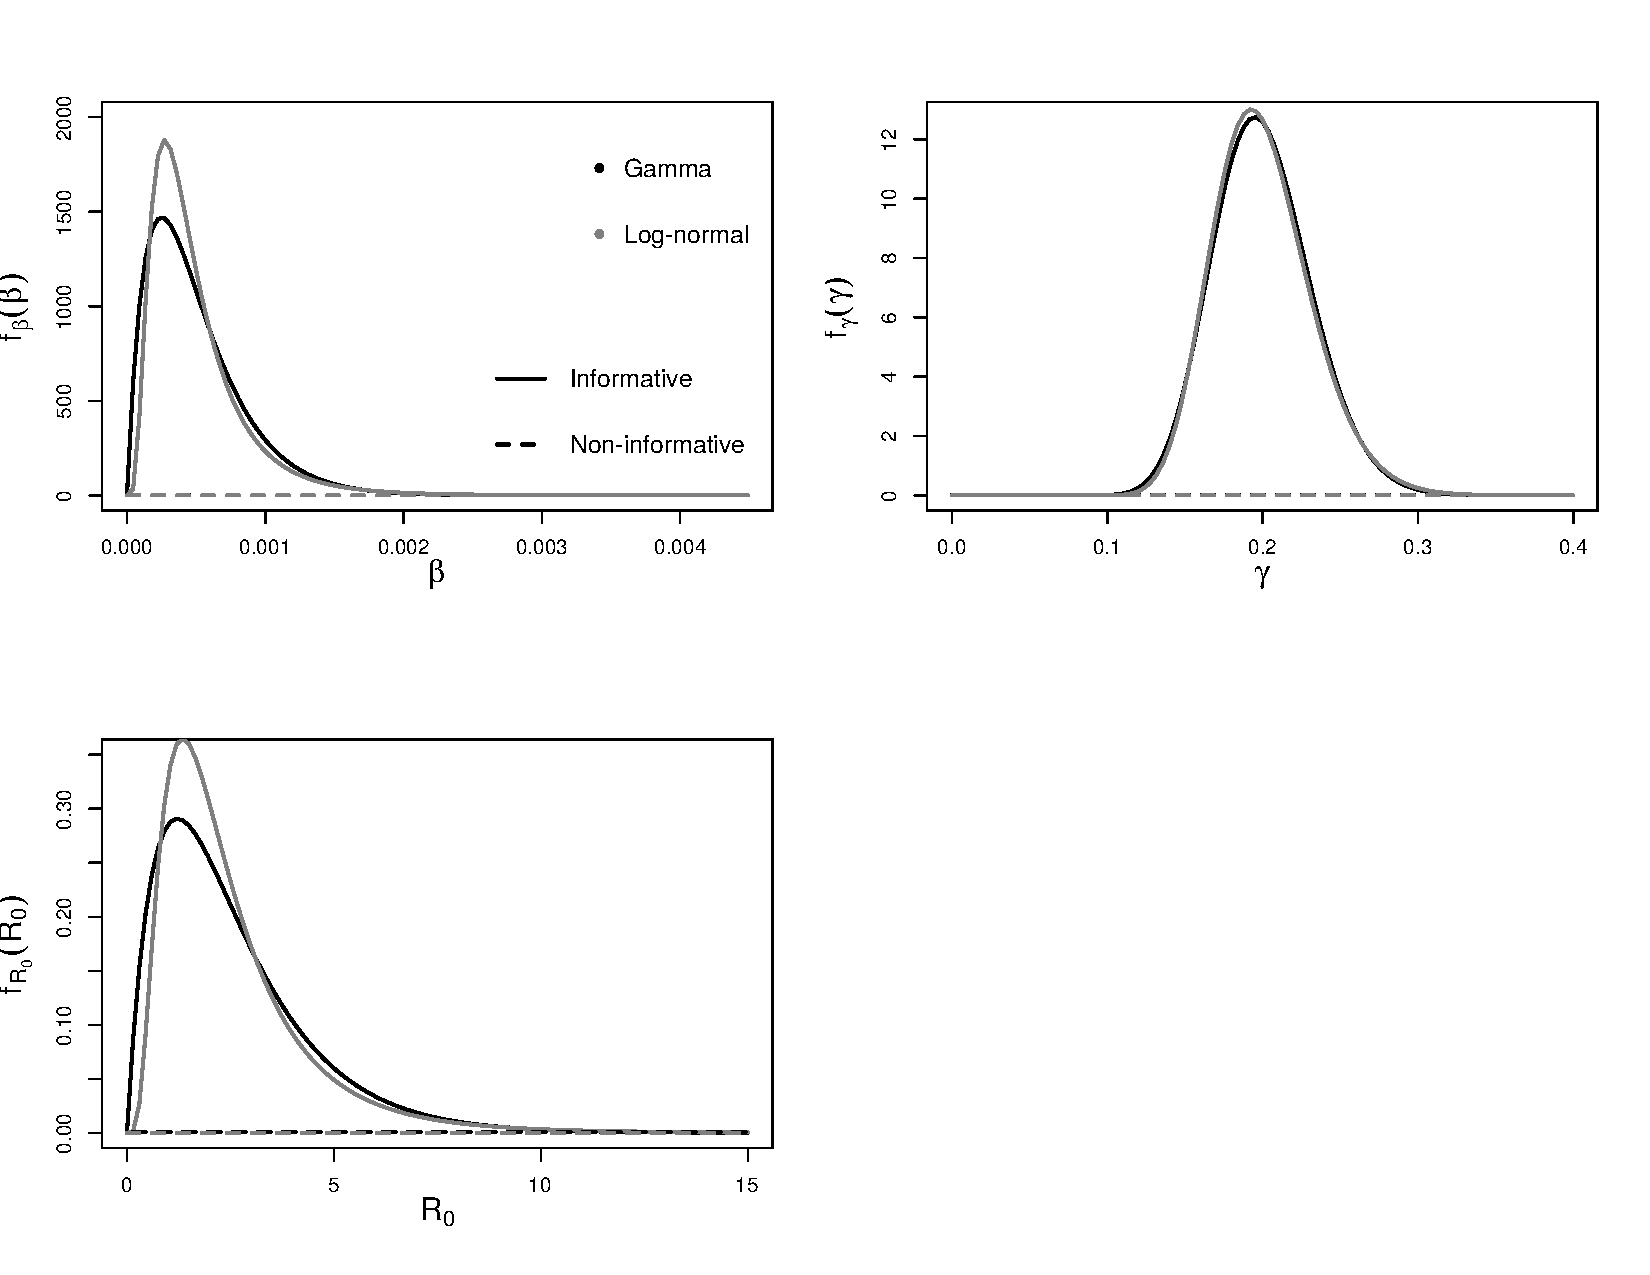
\includegraphics[scale=0.4]{figures/informative_example.pdf}
\caption{Informative and uninformative priors for the transmission ($\beta$) and recovery ($\gamma$) rates and the induced density on the basic reproductive number, $\rr$.
Solid lines show the informative prior, whilst dashed lines show the uninformative formulation (see text).
Black lines represent the Gamma priors (and Gamma ratio for $\rr$) and grey lines pertain to the moment-matching log-normal densities.}
\label{fig:informative_priors_example}
\end{figure}

\paragraph{Accounting for Biology}

The physical interpretation of $\rr$ is the number of secondary infections caused by a single infectious individual in a susceptible population.
This means that $\rr$ cannot exceed the population size $N$, which for simplicity we will assume is fixed through time.
One can obtain a distribution on $\rr$ with the correct bounds by correcting the distribution to have all of its probability mass in the interval $[0, N]$:
\begin{equation}
f_{\rr}^\prime(r \mid k_{\beta}, \theta_{\beta}, k_{\gamma}, \theta_{\gamma}, N) =  
 \begin{cases}
  \frac{1}{ F_{\rr}(N)} f_{\rr}(r \mid k_{\beta}, \theta_{\beta},  k_{\gamma}, \theta_{\gamma}, N ), \:  0 < r < N, \\
  0, \: \text{otherwise}
 \end{cases}
\end{equation}

% \begin{table}[bt]
% \caption{This is a table. Tables should be self-contained and complement, but not duplicate, information contained in the text. They should be not be provided as images. Legends should be concise but comprehensive – the table, legend and footnotes must be understandable without reference to the text. All abbreviations must be defined in footnotes.}
% \begin{threeparttable}
% \begin{tabular}{lccrr}
% \headrow
% \thead{Variables} & \thead{JKL ($\boldsymbol{n=30}$)} & \thead{Control ($\boldsymbol{n=40}$)} & \thead{MN} & \thead{$\boldsymbol t$ (68)}\\
% Age at testing & 38 & 58 & 504.48 & 58 ms\\
% Age at testing & 38 & 58 & 504.48 & 58 ms\\
% Age at testing & 38 & 58 & 504.48 & 58 ms\\
% Age at testing & 38 & 58 & 504.48 & 58 ms\\
% \hiderowcolors
% stop alternating row colors from here onwards\\
% Age at testing & 38 & 58 & 504.48 & 58 ms\\
% Age at testing & 38 & 58 & 504.48 & 58 ms\\
% \hline  % Please only put a hline at the end of the table
% \end{tabular}
% \begin{tablenotes}
% \item JKL, just keep laughing; MN, merry noise.
% \end{tablenotes}
% \end{threeparttable}
% \end{table}

\section*{Discussion}

~\citep{Weidemann2014} present skew normal priors as a more flexible approach to Gamma and Beta priors, since the SN has three parameters.
This makes it easier to construct priors from a point estimate of central tendency and confidence/credibility intervals.
%TODO 

\section*{Acknowledgements}
We would like to thank Erik Volz and Philip O'Neill for helpful discussions.

\section*{conflict of interest}
You may be asked to provide a conflict of interest statement during the submission process. Please check the journal's author guidelines for details on what to include in this section. Please ensure you liaise with all co-authors to confirm agreement with the final statement.

% \printendnotes

\section{Appendix}

To derive the induced distribution, we begin by noting that for $N > 1$, the distribution of $\beta^{\ast} = \beta N$ is a Gamma distribution with parameters $k_{\beta}$ and $N\theta_{\beta}$.
Under the assumption of independence $\pi(\beta^{\ast}, \gamma) = f_{\beta^\ast}(\beta^{\ast})f_{\gamma}(\gamma)$, we can write
\begin{eqnarray}
\rr &=& \beta^{\ast}/\gamma,\\
f_{\rr}(r) &=& A \int_{0}^{\infty} \gamma(\gamma r)^{k_{\beta} -1} e^{-\frac{\gamma r}{N\theta_{\beta}}} \gamma^{k_{\gamma} -1} e^{-\frac{\gamma}{\theta_{\gamma}}} d\gamma, \\
\nonumber
A &:=& \frac{1}{\Gamma(k_{\beta})(N\theta_{\beta})^{k_{\beta}}\Gamma(k_{\gamma})\theta_{\gamma}^{k_{\gamma}}}.
\end{eqnarray}
Rearranging yields
\begin{eqnarray}
\label{eq:toint}
f_{\rr}(r) &=& A  r^{k_{\beta} -1} \int_{0}^{\infty} \gamma^{k_{\beta} + k_{\gamma} -1} e^{-B\gamma} d\gamma, \\
\nonumber
        B  &:=& \frac{\theta_{\gamma} r + N\theta_{\beta}}{N\theta_{\beta}\theta_{\gamma}}.
\end{eqnarray}
Noticing the integral in (\ref{eq:toint}) is the kernel of a Gamma pdf gives the result in~(\ref{eq:density}).
For a two slightly different derivations, see~\cite{Coelho2007} for a calculation based on generalised Gamma distributions and~\cite{Clancy2008} for a similar derivation to ours, but using the shape/rate parametrisation of the Gamma distribution.

% Submissions are not required to reflect the precise reference formatting of the journal (use of italics, bold etc.), however it is important that all key elements of each reference are included.
\bibliography{R0}

% \graphicalabstract{example-image-1x1}{Please check the journal's author guildines for whether a graphical abstract, key points, new findings, or other items are required for display in the Table of Contents.}

\end{document}
